
\documentclass[12pt]{article}

\usepackage{../sbc-template}
\usepackage[utf8]{inputenc}
\usepackage[T1]{fontenc}

\usepackage{graphicx,url}
\usepackage{amsmath,amssymb}
\usepackage{bm}

\usepackage{microtype}
\usepackage{booktabs}
\usepackage{dblfloatfix}
\usepackage{multirow}
\usepackage[section]{placeins}
\usepackage{float}
\makeatletter
\AddToHook{begindocument/before}[normalsfcodes-init]{%
  \global\let\normalsfcodes\@empty
}
\makeatother
\usepackage[english]{babel}
\usepackage[hidelinks]{hyperref}

\usepackage{tabularx}
\usepackage{subcaption}

\begin{document}

\section{External Probe --- Google Trends}
\label{sec:external_probe}

Without external ground truth for Portuguese political semantic
change~\cite{schlechtweg-etal-2020-semeval}, we triangulate the frozen
55-lemma panel against an independent temporal proxy, \textbf{Google Trends
search-interest} for Brazil (2004--2023), retrieved via the Oxylabs SERP API.
This strategy follows the culturomics
tradition~\cite{michel-etal-2011-quantitative,scheffer-etal-2021-rationality}
of using public-attention series as a complementary signal, not as ground
truth. Google Trends measures \textbf{normalized search volume}, not lexical
usage or semantic displacement~\cite{rovetta-2021-reliability-google-trends},
so we interpret any alignment as \textbf{contextual resonance} rather than
validation.

For each panel lemma we derived three yearly movement features from the Google
series, namely mean absolute change ($\Delta_{\mathrm{abs}}$), standard
deviation ($\sigma$), and range. Table~\ref{tab:external_correlations} reports
Spearman rank correlations against internal drift scores.

\begin{table}[H]
    \centering
    \footnotesize
    \caption{Spearman $\rho$ between internal drift and Google Trends movement.
    \textbf{Bold} = $p < 0.05$.}
    \label{tab:external_correlations}
    \begin{tabularx}{\linewidth}{@{}l l >{\raggedleft\arraybackslash}X >{\raggedleft\arraybackslash}X >{\raggedleft\arraybackslash}X@{}}
        \toprule
        Method & Subset & $\Delta_{\mathrm{abs}}$ & $\sigma$ & Range \\
        \midrule
        Word2Vec & Full panel & $\bm{0.30}$ & $\bm{0.51}$ & $\bm{0.50}$ \\
        Word2Vec & Drift only & $0.08$ & $0.32$ & $0.26$ \\
        TF-IDF & Full panel & $-0.07$ & $\bm{-0.45}$ & $\bm{-0.41}$ \\
        TF-IDF & Drift only & $-0.26$ & $\bm{-0.54}$ & $\bm{-0.47}$ \\
        BERT($-1$) & Full panel & $0.06$ & $0.07$ & $0.01$ \\
        \bottomrule
    \end{tabularx}
\end{table}

\textbf{Word2Vec shows moderate positive correlation} with Google volatility on
the full panel ($\rho = 0.51$, $p < 0.001$ for $\sigma$), but this
\textbf{weakens to non-significant} within the drift-only subset ($\rho = 0.32$,
$p = 0.085$). The signal is driven mostly by separating drift candidates from
the flattest stable controls, not by rank-ordering within the drift list.
Group-level tests confirm this pattern, as Word2Vec drift terms have higher external
movement than controls (Mann--Whitney $p = 0.013$, Cliff's $\delta = 0.50$).
\textbf{TF-IDF correlates negatively} ($\rho = -0.45$, $p < 0.001$), meaning
TF-IDF-led candidates are on average \emph{less} externally salient than
controls, reinforcing that TF-IDF captures agenda-internal reweightings.
\textbf{BERT shows no correlation} ($|\rho| < 0.08$, $p > 0.59$).

The time-series overlays in Figure~\ref{fig:ts_overlays} illustrate what these
correlations look like at the term level. All series are $z$-standardized
within term and source to compare temporal shape, not magnitude.
\textit{Previd\^encia} and \textit{reforma} show \textbf{convergence}, with
Google search interest and internal drift spiking together around 2016--2019 in
alignment with the pension-reform and constitutional-amendment debates.
\textit{Sal\'ario} shows a \textbf{rising Google trend} that partially tracks
TF-IDF drift in later years. \textit{Interven\c{c}\~ao}, by contrast,
illustrates \textbf{divergence}, ranking among the top Word2Vec drift terms
with a sharp spike around 2018 yet Google search interest remains flat,
showing that discourse-internal neighborhood displacement need not surface as
public search behavior.

\begin{figure}[H]
    \centering
    \begin{subfigure}[b]{0.48\linewidth}
        \centering
        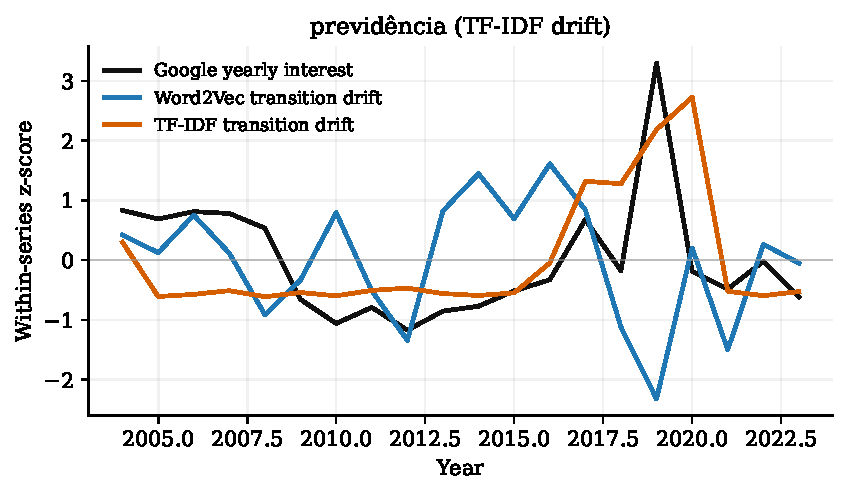
\includegraphics[width=\linewidth]{../figs/external/previdencia_google_vs_drift.pdf}
        \caption{\textit{previd\^encia} --- convergence}
    \end{subfigure}
    \hfill
    \begin{subfigure}[b]{0.48\linewidth}
        \centering
        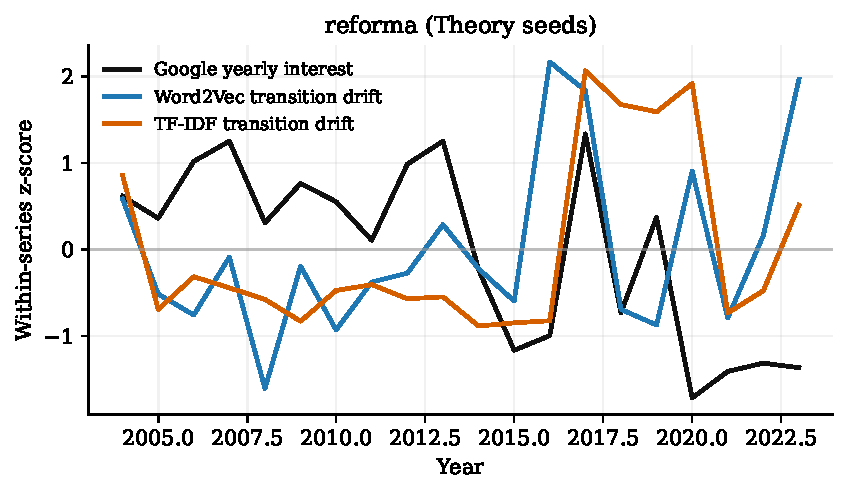
\includegraphics[width=\linewidth]{../figs/external/reforma_google_vs_drift.pdf}
        \caption{\textit{reforma} --- convergence}
    \end{subfigure}

    \vspace{4pt}

    \begin{subfigure}[b]{0.48\linewidth}
        \centering
        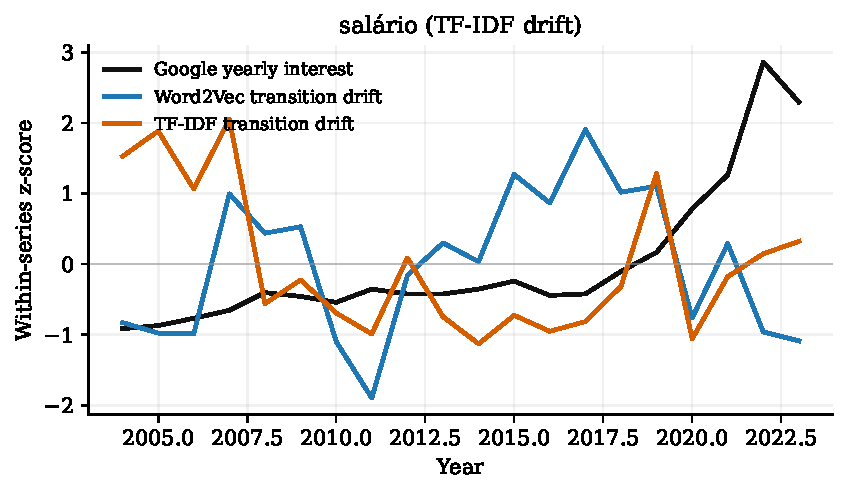
\includegraphics[width=\linewidth]{../figs/external/salario_google_vs_drift.pdf}
        \caption{\textit{sal\'ario} --- partial alignment}
    \end{subfigure}
    \hfill
    \begin{subfigure}[b]{0.48\linewidth}
        \centering
        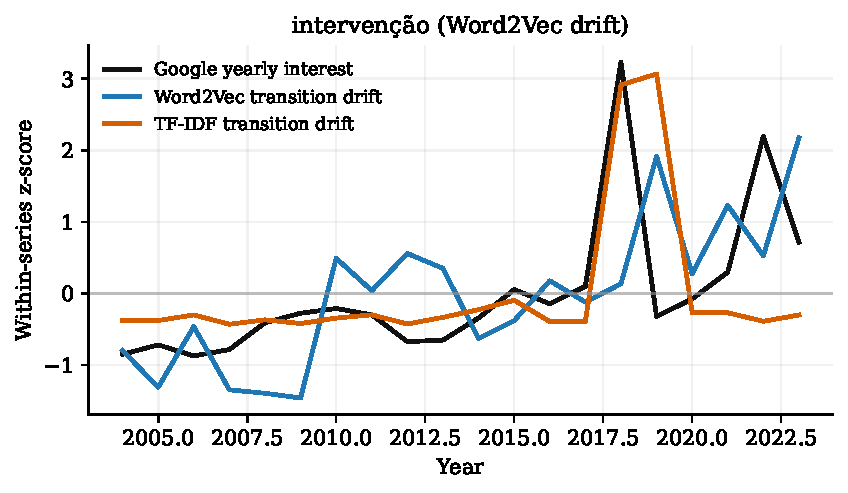
\includegraphics[width=\linewidth]{../figs/external/intervencao_google_vs_drift.pdf}
        \caption{\textit{interven\c{c}\~ao} --- divergence}
    \end{subfigure}

    \caption{Google Trends interest (black) vs.\ Word2Vec drift (blue) and
    TF-IDF drift (orange), $z$-scored per series. (a--b) show convergence for
    publicly salient terms; (c) partial alignment; (d) a top Word2Vec drift
    term with no Google echo.}
    \label{fig:ts_overlays}
\end{figure}

\subsection{Conclusion}
\label{sec:external_conclusion}

The Google Trends probe yields a clear answer. \textbf{There is no strong
external validation} of the frozen drift rankings. The relationship between
internal drift scores and public search-interest volatility is
\textbf{method-dependent, selective, and weak-to-moderate at best}.

Word2Vec drift is the only method that shows a positive association with Google
Trends movement ($\rho = 0.51$ on the full panel), but this correlation is
\textbf{driven by the gap between drift candidates and the flattest controls},
not by a monotonic relationship within the drift list itself. Once stable
controls are removed, the association drops to non-significant. TF-IDF drift
shows a \textbf{significant negative correlation}, meaning its top candidates
are \emph{less} publicly salient, not more. BERT shows \textbf{no relationship
at all}.

At the term level, the pattern is informative. Convergence occurs for
\textbf{publicly salient issue terms} such as \textit{previd\^encia},
\textit{reforma}, \textit{sa\'ude}, and \textit{sal\'ario}, where parliamentary
drift aligns with real-world policy debates that generate search attention.
Divergence occurs for \textbf{discourse-internal or bureaucratic terms}
(\textit{interven\c{c}\~ao}, \textit{juridicidade}) whose semantic
neighborhood shifts inside parliament leave no trace in public search behavior.

This selectivity is itself the main takeaway. Google Trends does not adjudicate
which drift detector is correct, but it confirms that the three methods
\textbf{capture fundamentally different facets of change}. Word2Vec picks up
publicly resonant neighborhood reorganizations, TF-IDF picks up
agenda-internal salience shifts that are invisible to Google, and BERT operates
at a usage level that a population-level search proxy simply cannot reach.
No single external signal benchmarks all three, reinforcing the paper's core
finding that \textbf{disagreement among methods is not noise --- it is
evidence that they measure different things}.

\bibliographystyle{../sbc}
\bibliography{../bib/bib_external_probe}

\end{document}
